\section{Экономическое обоснование проекта}

Проведём расчёт стоимости работ, связанных с разработкой
продукта ConfigtCastle и его дальнейшей эксплуатации.

\tocless\subsection{Экономическая концепция стартапа}

На рисунке \ref{ec:canvas} отображена общая экономическая составляющая стартапа.
Показаны способы привлечения клентов, статьи расходов и так далее.

\begin{figure}[H]
    \center{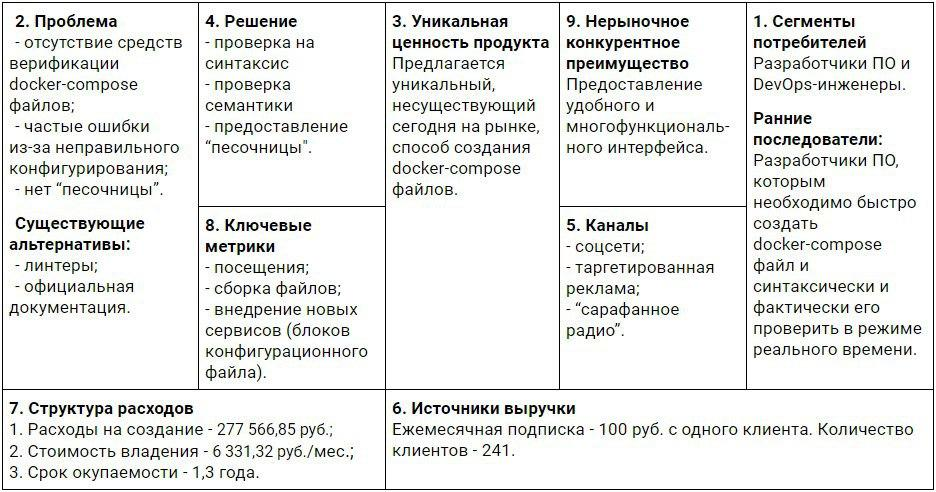
\includegraphics[scale=0.5]{canvas.jpg}}
    \caption{Экономическое описание стартапа}
    \label{ec:canvas}
\end{figure}

\tocless\subsection{Расчёт прямых расходов}

Прямые расходы включают в себя:
\begin{itemize}
    \item Расходы на оплату труда с учётом трудозатрат;
    \item Страховые взносы во внебюджетные фонды
\end{itemize}

\subsubsection{Расчёт расходов на оплату труда}

Разработкой проекта будут заниматься backend-разработчик и
frontend-разработчик.

Их заработная плата составляет по 20 000 руб. в месяц. Расчёт произведём по формуле \ref{ec:fot}

\begin{equation}
    \label{ec:fot}
    \text{ФОТ}_\text{год} = \text{ЗП} * 12 \text{мес},
\end{equation}

\begin{eqexpl}[5ex]
    \item{ФОТ} Фонд оплаты труда, руб.;
    \item{ЗП} Заработная плата, руб.;
\end{eqexpl}

\begin{equation*}
    \text{ФОТ}_\text{год} = 20 000 * 12 \text{мес.} = 240 000 \, \text{руб.}
\end{equation*}

Теперь определм стоимость трудозатрат в час по формуле \ref{ec:trudzat}:

\begin{equation}
    \label{ec:trudzat}
    \text{Ct}_\text{час} = \text{ФОТ} / N_\text{рв},
\end{equation}

\begin{eqexpl}[5ex]
    \item{$\text{Ct}_\text{час}$}  Стоимость трудозатрат за 1 час, руб
    \item{$\text{N}_\text{рв},$} Норма рабочего времени при 40-ка часовой рабочей
неделе.
\end{eqexpl}

\begin{equation*}
    \text{Ct}_\text{час} = 240 000 / 1979 = 121,27 \, \text{руб}.
\end{equation*}

Теперь рассчитаем сумму расходов на оплату труда и каждый пункт
разработки занесём в таблицу \ref{ec:table1}.

\tabcolsep=0.1cm
\begin{longtable}[c]{|l|c|c|r|}
    \caption{Расчет расходов на оплату труда с учетом трудозатрат}
    \label{ec:table1}\\
    \hline
    \multicolumn{1}{|c|}{{\begin{tabular}[c]{@{}c@{}}Наименование\\ работ/услуг\end{tabular}}} &
      {\begin{tabular}[c]{@{}c@{}}Трудозатраты, \\ час\end{tabular}} &
      {\begin{tabular}[c]{@{}c@{}}Стоимость \\ трудозатрат в час, \\ руб\end{tabular}} &
      {\begin{tabular}[c]{@{}c@{}}Общая стоимость\\ работ, \\ руб\end{tabular}} \\ \hline
    \endfirsthead
    %
    \multicolumn{4}{l}%
    {{\hspace{5ex} Продолжение таблицы \thetable \vspace{0.5cm}}} \\ \hline
    \multicolumn{1}{|c|}{{\begin{tabular}[c]{@{}c@{}}Наименование\\ работ/услуг\end{tabular}}} &
    {\begin{tabular}[c]{@{}c@{}}Трудозатраты, \\ час\end{tabular}} &
    {\begin{tabular}[c]{@{}c@{}}Стоимость \\ трудозатрат в час, \\ руб\end{tabular}} &
    {\begin{tabular}[c]{@{}c@{}}Общая стоимость\\ работ, \\ руб\end{tabular}} \\ \hline    \endhead
    %
    \begin{tabular}[c]{@{}l@{}}Разработка\\ требований\end{tabular}                              & 72            & 121,27          & 8731,44           \\ \hline
    \begin{tabular}[c]{@{}l@{}}Создание прототипов\\ пользовательского\\ интерфейса\end{tabular} & 16            & 121,27          & 1940,32            \\ \hline
    \begin{tabular}[c]{@{}l@{}}Написание прототипа\\ сервера\end{tabular}                        & 36            & 121,27          & 4365,72            \\ \hline
    Создание дизайна                                                                             & 32            & 121,27          & 3880,64            \\
    \pagebreak
    \begin{tabular}[c]{@{}l@{}}Разработка общей\\ архитектуры проекта\end{tabular}               & 56            & 121,27          & 6791,12           \\ \hline
    Выбор технологий                                                                             & 24            & 121,27          & 2910,48            \\ \hline
    \begin{tabular}[c]{@{}l@{}}Написание кода\\ клиентской части\end{tabular}                    & 496           & 121,27          & 60149,92           \\ \hline
    \begin{tabular}[c]{@{}l@{}}Написание кода\\ серверной части\end{tabular}                     & 456           & 121,27          & 55299,12           \\ \hline
    \begin{tabular}[c]{@{}l@{}}Тестирование клиентской\\ части\end{tabular}                      & 40            & 121,27          & 4850,80            \\ \hline
    \begin{tabular}[c]{@{}l@{}}Тестирование сервеной\\ части\end{tabular}                        & 24            & 121,27          & 2910,48            \\ \hline
    Написание документации                                                                       & 8             & 121,27          & 970,16            \\ \hline
    \begin{tabular}[c]{@{}l@{}}Изучение документаций к\\ выбранным технологиям\end{tabular}      & 24            & 121,27          & 2910,48            \\ \hline
    Развёртывание на сервере                                                                     & 24            & 121,27          & 2910,48            \\ \hline
    {Итого}                                                                                      & 1308          & 121,27          & 158621,16          \\ \hline
\end{longtable}

\subsubsection{Расчёт страховых взносов во внебюджетные фонды}

Следующим шагом будет определение страховых взносов во внебюджетные фонды, которые состоят
из следующих тарифов:

\begin{itemize}
    \item на обязательное пенсионное страхование ~--- 22,0\%;
    \item на обязательное социальное страхование на случай временной нетрудоспособности и в связи с материнством ~--- 2,9\%;
    \item на обязательное медицинское страхование ~--- 5,1\%;
    \item на обязательное социальное страхование от несчастных случаев на производстве и профессиональных заболеваний ~--- 0.2\%.
\end{itemize}

Для расчёта общих страховых взносов используется формула \ref{ec:strah}:

\begin{equation}
    \label{ec:strah}
    \text{C}_\text{страх-вз} = \text{ФОТ}_\text{год} * 30,2\% / 100\%,
\end{equation}

\begin{eqexpl}[7ex]
    \item{$\text{ФОТ}_\text{год}$} Фонд оплаты труда, руб.
\end{eqexpl}

\begin{equation*}
    \text{C}_\text{страх-вз} = 158621,16 * 30,2\% / 100\% = 47903,59 \, \text{руб}.
\end{equation*}

\tocless\subsection{Определение накладных расходов на разработку программного продукта}

Накладные расходы включают в себя следующие пункты:

\begin{itemize}
    \item Услуги связи(интернет, телефон);
    \item Коммунальные расходы;
    \item Расходы на рекламу;
    \item Прочие
\end{itemize}

Для расчёта накладных расходов рассчитаем временные сроки выполнения проекта по следующей
формуле:

\begin{equation}
    \text{СП} = \text{t}_\text{Общ} / 8,
\end{equation}

\begin{eqexpl}[5ex]
    \item{СП} Временные сроки выполнения, дн.;
    \item{$\text{t}_\text{общ}$} Общая сумма трудозатрат, час;
    \item{8} Стандартный рабочий день, час.
\end{eqexpl}

\begin{equation*}
    \text{СП} = 1308 / 8 = 163,5 \, \text{дн}.
\end{equation*}

\subsubsection{Расчёт расходов на услугуи связи}

Расчёт расходов на связь можно посчитать по следующей формуле:

\begin{equation}
    \text{P}_\text{y.c.} = (\text{P}_\text{интернет} + \text{P}_\text{тел.связь}) / \text{Кол-во дней(мес)} * \text{СП},
\end{equation}

\begin{eqexpl}[18ex]
    \item{$\text{P}_\text{интернет} + P_\text{тел.связь}$} Расходы на интернет, мобильную связь и т.д.;
    \item{Кол-во дней(мес)} Среднее количество рабочий дней в месяце, дн.
\end{eqexpl}

\begin{equation*}
    \text{P}_\text{y.c.} = (450 + 300 + 400 + 300) / 21 * 163,5 = 11289,29 \, \text{руб}.
\end{equation*}

\subsubsection{Расчёт расходов на коммунальные услуги}

Расчёт коммунальных услуг произведём по формуле \ref{ec:eq_com}:

\begin{equation}
    \label{ec:eq_com}
    \text{P}_\text{коммунальные} = \text{n}_\text{к.у} * \text{S} / \text{Кол-во дней(мес)} * \text{СП},
\end{equation}

\begin{eqexpl}[12ex]
    \item{$\text{P}_\text{коммунальные}$} Расходны на коммунальные услуги;
    \item{$\text{n}_\text{к.у}$} Средняя ставка на ком. услуги за 1 кв. метр;
    \item{$\text{S}$} Площадь помещения в кв. м.
\end{eqexpl}

\begin{equation*}
    \text{P}_\text{коммунальные} = 120 * 30 / 21 * 163,5 = 28028,57 \, \text{руб}.
\end{equation*}

\subsubsection{Расчёт расходов на рекламу}

Произведём расчёт расходов на рекламу по следующей формуле:

\begin{equation}
    \text{P}_\text{реклама} = \text{POT} * \text{n}_\text{реклама} / 100\%,
\end{equation}

\begin{eqexpl}[7ex]
    \item{$\text{P}_\text{реклама}$} Сумма расходов на рекламу, руб.;
    \item{$\text{POT}$} Расходы на оплату труда, руб.;
    \item{$\text{n}_\text{реклама}$} Норматив расходов на рекламу, руб.
\end{eqexpl}

\begin{equation*}
    \text{P}_\text{реклама} = 158621,16 * 10\% / 100\% = 15862,12 \, \text{руб}.
\end{equation*}

\subsubsection{Расчёт прочих расходов}

Рассчитаем расходы на оплату труда, которые являются процентом от расходов
на оплату труда как и расходы на рекламу, по формуле:

\begin{equation}
    \text{P}_\text{прочие} = \text{POT} * \text{n}_\text{прочие} / 100\%,
\end{equation}

\begin{eqexpl}[6ex]
    \item{$\text{P}_\text{прочие}$} Сумма прочих расходов, руб.;
    \item{$\text{n}_\text{прочие}$} Норматив прочих расходов, \%
\end{eqexpl}

\begin{equation*}
    \text{P}_\text{прочие} =  158621,16 * 10\% / 100\% = 15862,12 \text{руб}.
\end{equation*}

\subsubsection{Расчёт общей суммы накладных расходов}

Теперь можно определить общую сумма накладных расходов по формуле \ref{ec:nak}:

\begin{equation}
    \label{ec:nak}
    \text{P}_\text{Накладные} = \text{P}_\text{y.c.} + \text{P}_\text{коммунальные} + \text{P}_\text{реклама} + \text{P}_\text{прочие}.
\end{equation}

\begin{eqexpl}[9ex]
    \item{$\text{P}_\text{Накладные}$} Сумма накладных расходов, руб.
\end{eqexpl}

\begin{equation*}
    \text{P}_\text{Накладные} = 11289,29 + 3600 + 15862,12 * 2 = 71042,10 \, \text{руб.}
\end{equation*}

\tocless\subsection{Расчёт себестоимости работ по разработке программного продукта}

Себестоимость работ по проекту включает в себя:

\begin{itemize}
    \item Расходы на оплату труда;
    \item Страховые взносы;
    \item Накладые расходы.
\end{itemize}

Расчёт себестоимости работ по проекту, иными словами цену непосредственного создания
программного продукта, привидена в таблице \ref{ec:table2}.

\begin{longtable}[c]{|p{10cm}|r|}
    \caption{Себестоимость работ по созданию программного продукта}
    \label{ec:table2}\\
    \hline
    \multicolumn{1}{|c|}{{Статьи расходов}} & {\begin{tabular}[c]{@{}c@{}}Сумма, руб.\end{tabular}} \\ \hline
    \endfirsthead
    %
    \multicolumn{2}{c}%
    {{Продолжение таблицы \thetable}} \\
    \endhead
    %
    Расход на оплату труда & 158621,16          \\ \hline
    Страховые взносы       & 47903,59           \\ \hline
    Накладные расходы      & 71042,10           \\ \hline
    {Итого}         & 277566,85 \\ \hline
\end{longtable}

\tocless\subsection{Расчёт стоимости владения программным продуктом}

Стоимость владени программным продуктом включает в себя
эксплуатационные расходы (Эр) на обслуживание разработанного
программного продукта (таблица \ref{ec:table5}), измеряются в часах, затраченных на
указанные ниже виды работ.

Ежемесячные затраты на функционирование (Зф) программного
продукта (таблица \ref{ec:table6}) так же входят в стоимость владения программным
продуктом.

\tabcolsep=0.1cm
\begin{longtable}[c]{|l|c|c|r|}
    \caption{Расчет эксплуатационных расходов.
    }
    \label{ec:table5}\\
    \hline
    \multicolumn{1}{|c|}{{Наименование статей}} &
      \begin{tabular}[c]{@{}c@{}}Количество\\ часов,\\ час/мес\end{tabular} &
      \begin{tabular}[c]{@{}c@{}}Стоимость\\ трудозатрат в\\ час, \\ руб.\end{tabular} &
      \begin{tabular}[c]{@{}c@{}}Сумма,\\ руб. в месяц\end{tabular} \\ \hline
    \endfirsthead
    %
    \multicolumn{4}{c}%
    {{Продолжение таблицы \thetable}} \\
    \endhead
    %
    Наполнение контентом                                                                                         & 16          & 121,27          & 1940,32           \\ \hline
    Оптимизация производительсности                                                                                 & 8          & 121,27          & 970,16            \\ \hline
    \begin{tabular}[c]{@{}l@{}}Установка и тестирование\\ программных обновлений\\ разработотанного ПО\end{tabular} & 5           & 121,27          & 606,35            \\ \hline
    Модерация ресурсов                                                                                              & 16          & 121,27          & 1940,32            \\ \hline
    Итого                                                                                                  & 45 & 181.91 & 5457,15 \\ \hline
\end{longtable}

\begin{longtable}[c]{|p{10cm}|r|}
    \caption{Расчет затрат на функционирование.
    }
    \label{ec:table6}\\
    \hline
    \multicolumn{1}{|c|}{{Виды затрат}}                                              & \begin{tabular}[c]{@{}c@{}}Сумма,\\ руб./месяц\end{tabular} \\ \hline
    \endfirsthead
    %
    \multicolumn{2}{c}%
    {{Продолжение таблицы \thetable}} \\
    \endhead
    %
    Стоимость домена   & 49,17           \\ \hline
    Стоимость хостинга & 825,00           \\ \hline
    {Итого}     & {874,17} \\ \hline
\end{longtable}

Итого, стоимость владения (Св) рассчитывается как сумма
эксплуатационных расходов и затрат на функционирование по формуле \ref{ec:st_vl}:

\begin{equation}
    \label{ec:st_vl}
    \text{C}_\text{в} = \text{Э}_\text{р} + \text{З}_\text{ф}.
\end{equation}

\begin{equation*}
    \text{C}_\text{в} = 5457,15 + 874,17 = 6 331,32 \, руб.
\end{equation*}

Вывод: стоимость владения разработанным продуктом, составляет 6 331,32 руб. в месяц.

\vspace{1.2cm}

\tocless\subsection{Смета затрат на проект}

Смета затрат на проект включает в себя себестоимость проекта,
заложенную сумму прибыли разработчика, сумму налоговых платежей.
Отдельной строкой необходимо указать стоимость владения программным
продуктом. Расчёт сметы представлен в таблице \ref{ec:table7}

\begin{longtable}[c]{|c|p{11.5cm}|r|}
    \caption{Смета затрат на проект.}
    \label{ec:table7}\\
    \hline
    \multicolumn{1}{|c|}{{\begin{tabular}[c]{@{}c@{}}№\\ п/п\end{tabular}}} &
      \multicolumn{1}{c|}{{Статьи смета затрат на проект}} &
      {\begin{tabular}[c]{c@{}c@{}}Сумма, руб.\end{tabular}} \\ \hline
    \endfirsthead
    %
    \multicolumn{3}{l}{Продолжение таблицы \thetable \vspace{0.5cm}} \\ \hline
    \multicolumn{1}{|c|}{{\begin{tabular}[c]{@{}c@{}}№\\ п/п\end{tabular}}} &
    \multicolumn{1}{c|}{{Статьи смета затрат на проект}} &
    {\begin{tabular}[c]{@{}c@{}}Сумма, руб.\end{tabular}} \\ \hline
    \endhead
    %
    1 &
      \begin{tabular}[c]{@{}l@{}}Затратны на создание программного продукта\\ (себестоимость работ)\end{tabular} &
      277566,85 \\ \hline
    2                    & Стомость владения ПП, месяц           & 6331,32   \\ \hline
\end{longtable}

\vspace{1.5cm}

\tocless\subsection{Расчёт сроков окупаемости}

Первым делом была рассчитана предположительная ежемесячная
посещаемость сервиса. Было взято наименьшее число посетителей среди
существующих на рынке похожих сервисов. Минимум был взят в связи с
тем, что исследуемы сервисы уже укоренились на рынке, а в случае с
проектом «configCastle», этот процесс ещё только планируется. Это число
составило 2 500 в месяц (сервис https://scriptular.com/).

Далее, требуется рассчитать долю клиентов среди посетителей. Для
этого обратимся к анкете.

На вопрос «Часто ли вы имеете дело с файлом docker-compose.yaml?»
(вопрос №1), ответ «Часто» дало 13\% анкетируемых. Умножим этот процент
на процент тех, кто дал ответ «Да» на вопрос: «Хотели бы вы иметь под
рукой графический интерфейс со множеством возможностей для
редактирования docker-compose.yaml?» (вопрос №2), то есть на 74%. В
результате, мы получим приблизительную долю клиентов среди всех
посетителей. Расчёты проведём по формуле \ref{ec:dol_client}.

\begin{equation}
    \label{ec:dol_client}
    \text{Доля клиентов} = \text{Вопрос №1} * \text{Вопрос №2},
\end{equation}

\begin{eqexpl}[15ex]
    \item{Доля клиентов} доля клиентов среди посетителей;
    \item{Вопрос №1} процент ответивших "<Часто"> на вопрос №1;
    \item{Вопрос №2} процент ответивших "<Да"> на вопрос №2; 
\end{eqexpl}

\begin{equation*}
    \text{Доля клиентов} = 0,13 * 0,74 = 0,0962.
\end{equation*}

Далее, рассчитаем количество клиентов, которые будут использовать
продукт ежемесячно. Для этого выполним расчёт по формуле \ref{ec:col_client}.

\begin{equation}
    \label{ec:col_client}
    \text{Кол-во клиентов} = \text{Кол-во посетителей} * \text{Доля клиентов},
\end{equation}

\begin{eqexpl}[19ex]
    \item{Кол-во посетителей}  предполагаемое количество посетителей за
    месяц, человек.
    \item{Кол-клиентов} количество клиентов среди посетителей сервиса,
    человек;
\end{eqexpl}

\begin{equation*}
    \text{Кол-во клиентов} = 2 500 * 0,0962 = 241.
\end{equation*}

Стоимость владения проектом составляет 6 331,32 руб. в месяц. Для
расчёта стоимости ежемесячной подписки, для начала вычислим
минимальную сумму, требующуюся для покрытия расходов ($\text{C}_\text{min}$) по
формуле \ref{ec:c-min}.

\begin{equation}
    \label{ec:c-min}
    \text{C}_\text{min} = \text{Ст.владения} / \text{Кол-во клиентов},
\end{equation}

\begin{eqexpl}[13ex]
    \item{Ст. владения} стоимость владения продуктом.
\end{eqexpl}

\begin{equation*}
    \text{C}_\text{min} = 6 331,32 / 241 = 26,27 \text{руб}.
\end{equation*}

С учётом планов по окупаемости проекта и дальнейшего его развития,
стоит повысить эту сумму до 100 рублей ($\text{С}_\text{назнач}.$).

Следующий этап расчёта сроков окупаемости – суммы расчёт
ежегодной выручки ($\text{В}_\text{год}$), который проведём по формуле \ref{ec:year}:

\begin{equation}
    \label{ec:year}
    \text{В}_\text{год} = \text{С}_\text{назнач} * \text{Кол-во клиентов} * \text{Кол-во месяцев},
\end{equation}

\begin{eqexpl}[16ex]
    \item{Кол-во месяцев} количество месяцев в году.
\end{eqexpl}

\begin{equation*}
    \text{В}_\text{год} = 100 * 241 * 12 = 289200 \, \text{руб}.
\end{equation*}

Далее рассчитаем ежегодные расходы на владение продуктом ($\text{Р}_\text{год}$) по
формуле \ref{ec:r_year}:

\begin{equation}
    \label{ec:r_year}
    \text{Р}_\text{год} = \text{Ст. владения} * \text{Кол-во месяцев},
\end{equation}

\begin{equation*}
    \text{Р}_\text{год} =  6 331,32 × 12 = 75 975,84 \, \text{руб}.
\end{equation*}

Наконец, определим срок окупаемости проекта по формуле \ref{ec:sroc_oc}:

\begin{equation}
    \label{ec:sroc_oc}
    \text{Срок окупаемости} = \text{Ср} / (\text{В}_\text{год} - \text{Р}_\text{год}).
\end{equation}

\begin{equation*}
    \text{Срок окупаемости} = 277 566,85 / (289 200 - 75 975,84) = 1,3 \, \text{года}.
\end{equation*}
